\documentclass[options]{beamer}
\usepackage{graphicx}

\usetheme{Madrid}
\usecolortheme{crane}
\title{Moogle!}
\author{Lia S. López Rosales}
\titlegraphic{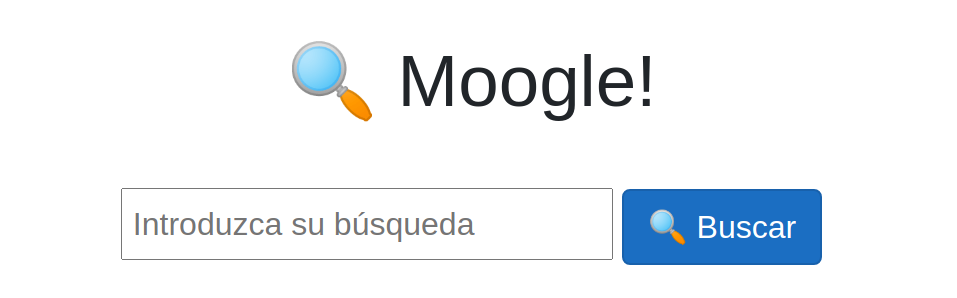
\includegraphics[width=4.5cm,height=1.5cm]{moogle.png}}
\begin{document}
\frame{\titlepage}
\begin{frame}{Moogle?}
    \begin{columns}[t]
        \begin{column}{.5\textwidth}
            \begin{center}
                \textbf{\Large Qué es?}\\
                \emph{Moogle es un buscador sintáctico local que trabaja sobre un conjunto de datos especificados por el usuario}
            \end{center}
        \end{column}
    \end{columns}
    
\end{frame}

\begin{frame}{Funcionamiento}
    \Large Mientras que en la presentación no se abordará en detalle todo el funcionamiento de la aplicación si se hablará sobre su algoritmo base el cual es ni más ni menos que la búsqueda vectorial, específicamente, el algoritmo conocido como TF-IDF ( Term Frecuency and Inverse Document Frecuency) cuya base se encuentra en la abstracción de los documentos y palabras como vectores y valores respectivamente. 
\end{frame}

\begin{frame}{Más sobre TF-IDF}
    \begin{itemize}
        \item TF ( Term Frecuency) se traduce como la abstracción de otorgarle a cada palabra un valor numérico, justamente su frecuencia, en el vector del documento 
        \item IDF ( Inverse Document Frecuency) este sin embargo otorga a cada palabra en valor en dependencia de que tan común es el universo de documentos donde se esté trabajando
        \item TF-IDF el resultado final de estos procesos se ve reflejado como el vector que representa al documento y que caracteriza a cada una de sus palabras. Lo que permite posteriormente obtener su relevancia según la búsqueda efectuada ( mediante otro algoritmo llamado similitud de cosenos)
    \end{itemize}
\end{frame}

\begin{frame}{Qué ofrece Moogle!?}
    \begin{enumerate}
        \item Búsqueda léxica en función de un conjunto de términos ingresados ( estos pueden tener sentido como conjunto o no tener nada en común) donde se obtiene una lista de los documentos relacionados a esta búsqueda según se relevancia ( ordenados de forma descendente)
        \item Recomendaciones sobre posibles búsquedas ( Sugerencias ) las cuales se muestran si alguno de los términos es inexistente en el conjunto de documentos pero se encuentran coincidencias con términos semejantes ( útil en caso de que haya ocurrido algún error ortográfico al ingresar la búsqueda)
        \item Más opciones de búsqueda(Operadores) para aumentar la precisión de la misma y filtrar resultados irrelevantes para el usuario
    \end{enumerate}
\end{frame}
\begin{frame}{Sugerencias}
    \begin{itemize}
        \item Este sistema del buscador permite al usuario obtener resultados a pesar de los posibles errores léxicos que se hallen en la búsqueda pues si no se encuentra el término se efectúa el proceso con el término semejante como sustituto
        \item Este por supuesto no es exacto y es posible que el término identificado como posible valor no sea el que el usuario pretendía encontrar ( está situación se vuelve más posible si la cantidad de errores o diferencias es mayor)
        \item Si en los documentos no se encuentra ninguna palabra semejante al término o si todos los términos de la búsqueda existen entonces se informará de ello al usuario en la sección de sugerencias y se procederá a efectuar el proceso habitual
    \end{itemize}
\end{frame}

\begin{frame}{Operadores}
    \begin{enumerate}
        \item Potenciación ($\ast $) permite declarar que tan relevante es la palabra en la búsqueda y por tanto para el usuario. Por lo que se otorgará mayor importancia a los documentos donde predomine el término
        \item Exclusión (!) permite declarar qué términos deben ser filtrados a la hora de entregar los resultados. Los documentos que contengan alguno de ellos serán considerados irrelevantes y por tanto no se mostrarán
        \item Inclusión (\textasciicircum) permite declarar qué términos son imprescindibles en la búsqueda, basado en esto se descartará cualquier documento que no contenga alguno de ellos
        \item Cercanía (\textasciitilde) permite declarar qué tan  relacionadas deberían estar las palabras (evaluar está situación es un poco ambiguo en una búsqueda puramente léxica por lo que se asume que existe una relación si los términos se encuentran en un mismo ámbito y por tanto se otorga mayor importancia a los documentos donde se encuentren más cerca las palabras)
    \end{enumerate}
\end{frame}

\begin{frame}{Más Información}
    \begin{itemize}
        \item Si se desea conocer a mayor profundidad el funcionamiento de la aplicación se puede consultar el informe adjunto a la misma donde se abordan todos los procesos que utiliza Moogle!
        \item También resulta útil consultar el informe para conocer condiciones específicas para emplear los operadores(ejemplo: síntaxis inválida)
    \end{itemize}
\end{frame}

\begin{frame}{"}
    \begin{center}
        \emph{\Huge Gracias}
    \end{center}
\end{frame}

\end{document}